\documentclass[conference,a4paper]{IEEEtran}

% Escritura mejorada de fórmulas matemáticas
\usepackage{amsmath}

\usepackage{float}


% Inserción de gráficos
\usepackage{graphicx}

% Escritura de pseudocódigo
\usepackage[kw]{pseudo}

% Escritura mejorada de tablas
\usepackage{booktabs}

% Escritura mejorada de citas bibliográficas
\usepackage{cite}


% Macros traducidas
\def\contentsname{Índice general}
\def\listfigurename{Índice de figuras}
\def\listtablename{Índice de tablas}
\def\refname{Referencias}
\def\indexname{Índice alfabético}
\def\figurename{Fig.}
\def\tablename{TABLA}
\def\partname{Parte}
\def\appendixname{Apéndice}
\def\abstractname{Resumen}
% IEEE specific names
\def\IEEEkeywordsname{Palabras clave}
\def\IEEEproofname{Demostración}


\begin{document}

\title{Algoritmos genéticos para problemas de regresión no lineal}

\author{
  \IEEEauthorblockN{Javier Ruíz Garrido}
  \IEEEauthorblockA{
    \textit{Dpto. Ciencias de la Computación e Inteligencia Artificial}\\
    \textit{Universidad de Sevilla}\\
    Sevilla, España\\
    2210jrg@gmail.com | javruigar2@alum.us.es}
  
  \and
  
  \IEEEauthorblockN{Javier Santos Martín}
  \IEEEauthorblockA{
    \textit{Dpto. Ciencias de la Computación e Inteligencia Artificial}\\
    \textit{Universidad de Sevilla}\\
    Sevilla, España\\
    javier.jsm21@gmail.com | javsanmar5@alum.us.es}
}

\maketitle


% Resumen
\begin{abstract}  
El objetivo principal de este trabajo fue desarrollar y evaluar un modelo de regresión no lineal utilizando algoritmos genéticos. Estos algoritmos, inspirados en los procesos de selección natural y evolución biológica, fueron empleados para optimizar los parámetros del modelo, representados en forma de cromosomas que contienen coeficientes y exponentes. Se realizaron experimentos con tres conjuntos de datos distintos: \texttt{toy1}, \texttt{housing} y \texttt{synt1}, evaluando el desempeño del modelo mediante el cálculo del error cuadrático medio (RMSE) y el coeficiente de determinación (R2).

El algoritmo creado cuenta con distintas ideas clave que fueron dando mejoras de rendimiento y precisión. Además, el control de la semilla de aleatoriedad y un sistema de registro de récords han sido muy importantes para garantizar los mejores resultados posibles del algoritmo. Entre las mejoras futuras, se sugiere paralelizar partes del código y aplicar este algoritmo en conjuntos de datos más grandes y complejos para validar su robustez y generalizabilidad.
\end{abstract}


% Palabras claves
\begin{IEEEkeywords}
    Algoritmo genético, regresión no lineal, cromosoma, mutación, cruce, elitismo.
\end{IEEEkeywords}


\section{Introducción}

En el campo de la inteligencia artificial y el aprendizaje automático, los algoritmos genéticos se han destacado como una poderosa herramienta para resolver problemas de optimización y búsqueda en espacios complejos. Estos algoritmos, inspirados en los procesos de selección natural y evolución biológica, se aplican a una variedad de dominios, desde la ingeniería hasta la economía, proporcionando soluciones efectivas donde otros métodos tradicionales pueden fallar. Los problemas de regresión no lineal, en particular, presentan desafíos significativos debido a la naturaleza intrínseca de sus relaciones no lineales entre variables. La búsqueda de modelos precisos y eficientes para estas relaciones es crucial en muchas aplicaciones prácticas, como la predicción financiera, la modelización de sistemas físicos y la medicina.

La problemática central de este proyecto radica en la precisión insuficiente de los métodos tradicionales de regresión lineal para modelar relaciones no lineales complejas en conjuntos de datos. El objetivo es desarrollar un modelo de regresión no lineal más preciso mediante el uso de algoritmos genéticos. La solución implementada se basa en la creación de cromosomas que representan coeficientes y exponentes para cada característica del conjunto de datos. Estos cromosomas son evaluados utilizando el error cuadrático medio (RMSE) como métrica de aptitud. El algoritmo genético itera sobre una población de cromosomas, aplicando operadores de selección por torneo, cruce y mutación, para optimizar los parámetros del modelo. El enfoque permite explorar de manera eficiente el espacio de búsqueda y ajustar los coeficientes y exponentes para minimizar el RMSE, mejorando así la capacidad del modelo de predecir futuros ejemplos.

El documento está estructurado de la siguiente manera: Tras la introducción, en la Sección II se describen los fundamentos teóricos con los que se ha trabajado el algoritmo genético y la regresión no lineal. La Sección III detalla la metodología propuesta, incluyendo la representación de los cromosomas, los operadores genéticos utilizados y el proceso de evaluación de los modelos. En la Sección IV se presentan los experimentos realizados y los resultados obtenidos, destacando las ventajas y limitaciones del enfoque propuesto. Finalmente, en la Sección V se presentan las conclusiones y se sugieren posibles líneas de investigación futura.

\section{Preliminares}
~\label{sec: preliminares}

En este trabajo, se busca aplicar la idea de los algoritmos genéticos para resolver problemas de regresión. Para ello, los cromosomas modelarán los parámetros de la función que intentamos predecir, y su valoración se realizará utilizando datos de prueba. Esto se llevará a cabo prediciendo los datos y evaluando la precisión de las predicciones comparándolas con los resultados esperados.

Todo esto se desarrollará dentro de un algoritmo genético estándar, que incluirá componentes como el elitismo, el cruce entre cromosomas y la mutación aleatoria. Finalmente, se explicarán algunas medidas para mejorar la eficiencia en este contexto específico.

\subsection{Cromosoma}

En el contexto de nuestro trabajo, el cromosoma se ha conceptualizado como una clase de Python. Para ello, se ha diseñado una clase abstracta denominada \textit{AbstractChromosome}, la cual establece los métodos fundamentales que debe poseer cualquier cromosoma. A partir de esta clase abstracta, se permite definir nuevas clases de cromosomas que extienden sus funcionalidades. En nuestro caso, hemos implementado la clase \textit{Chromosome(AbstractChromosome)}, la cual se ajusta a nuestros requerimientos, dado que podemos enmarcar todos los problemas de regresión no lineal en ella, sin tener que crear una clase distinta para cada fichero o problema a resolver.

El modelado del cromosoma en nuestro caso incluye los siguientes aspectos:

\subsubsection{Propiedades}
\begin{itemize}
    \item \textbf{Lista de coeficientes:} Esta lista contiene \( n + 1 \) elementos de tipo \texttt{float}, donde \( n \) es el número de variables independientes. El elemento \( j \) de la lista representa el coeficiente de la variable \( x_j \), mientras que el último elemento representa el término independiente.
    \item \textbf{Lista de exponentes:} Esta lista contiene \( n \) elementos de tipo \texttt{float}, donde \( n \) es el número de variables independientes. El elemento \( j \) de la lista representa el exponente de la variable \( x_j \).
\end{itemize}

Aunque, a priori, todos los elementos de ambas listas no tienen restricciones en cuanto a los valores que pueden adoptar, existen dos situaciones que podrían limitar estos valores:


1. \textbf{Variable \( x_i \) negativa:} En este caso, el exponente de la función no puede asumir valores fraccionarios cuyo denominador sea par, es decir, de la forma \( k/m \) donde \( m \) es par, en el ámbito de los números reales. A priori, este sería el único problema, pero obtenemos otro por la forma de trabajar de Python con las potencias fraccionarias: cualquier número negativo elevado a una potencia fraccionaria, ya sea con un denominador par o impar, resulta en un número complejo. Esto no es deseable, dado que estamos trabajando en el conjunto de los números reales. Podemos ver este fallo de Python ejemplificado a continuación, donde se eleva un número negativo \( -1 \) a un número fraccionario con denominador impar \( 0.2 = \frac{1}{5} \), lo que resulta en la raíz quinta de \(-1\), que es igual a \(-1\):

Esperado:
\[
\sqrt[5]{-1} = -1
\]

Obtenido:
\begin{verbatim}
>>> base, exponent = -1, 0.2
>>> base ** exponent
(0.8090169943749475+0.5877852522924731j)
\end{verbatim}

Hemos planteado diversas opciones para la resolución de este problema, como intentar modificar la fracción para garantizar que el denominador sea impar (lo cual hemos observado que no es efectivo debido al error en Python) o alterar la base (representada por la variable \(x_j\)), lo cual consideramos completamente incorrecto. Modificar la base implicaría permitir exponentes que generan este problema y exigiría a quienes utilicen esta solución que ajusten sus variables para trabajar con números positivos. Además, sabemos que si alteramos la base, es decir, los datos de entrada, el valor esperado \(y_i\) ya no sería válido, dado que el dato de entrada no sería el original. 


La alternativa seleccionada como solución al problema consiste en utilizar el módulo del resultado de la operación \(x_j^{e_j}\), ya que el error en Python parece ser un problema de aproximación. A continuación, se muestra que el módulo del número complejo devuelto es el mismo que el módulo del valor esperado (1):

\begin{verbatim}
>>> base, exponent = -1, 0.2
>>> base ** exponent
(0.8090169943749475+0.5877852522924731j)
>>> res = base ** exponent
>>> res
(0.8090169943749475+0.5877852522924731j)
>>> abs(res)
1.0
\end{verbatim}

Lo único que se requiere es multiplicar este valor por la función signo de la base (\(\text{sign}(x_j)\)). Esto se justifica de la siguiente manera: en el contexto de los números complejos, el número de soluciones a una raíz de índice \(i\) es igual a \(i\), y todas estas soluciones comparten una característica común: el módulo de estas soluciones es idéntico, y todas están espaciadas por el mismo ángulo entre ellas: \(\frac{360}{i}\). Véase la imagen \figurename~\ref{fig:roots_example}.

Esta solución ha proporcionado, además, los mejores resultados en nuestras pruebas.


\begin{figure}[H]
    \centering
    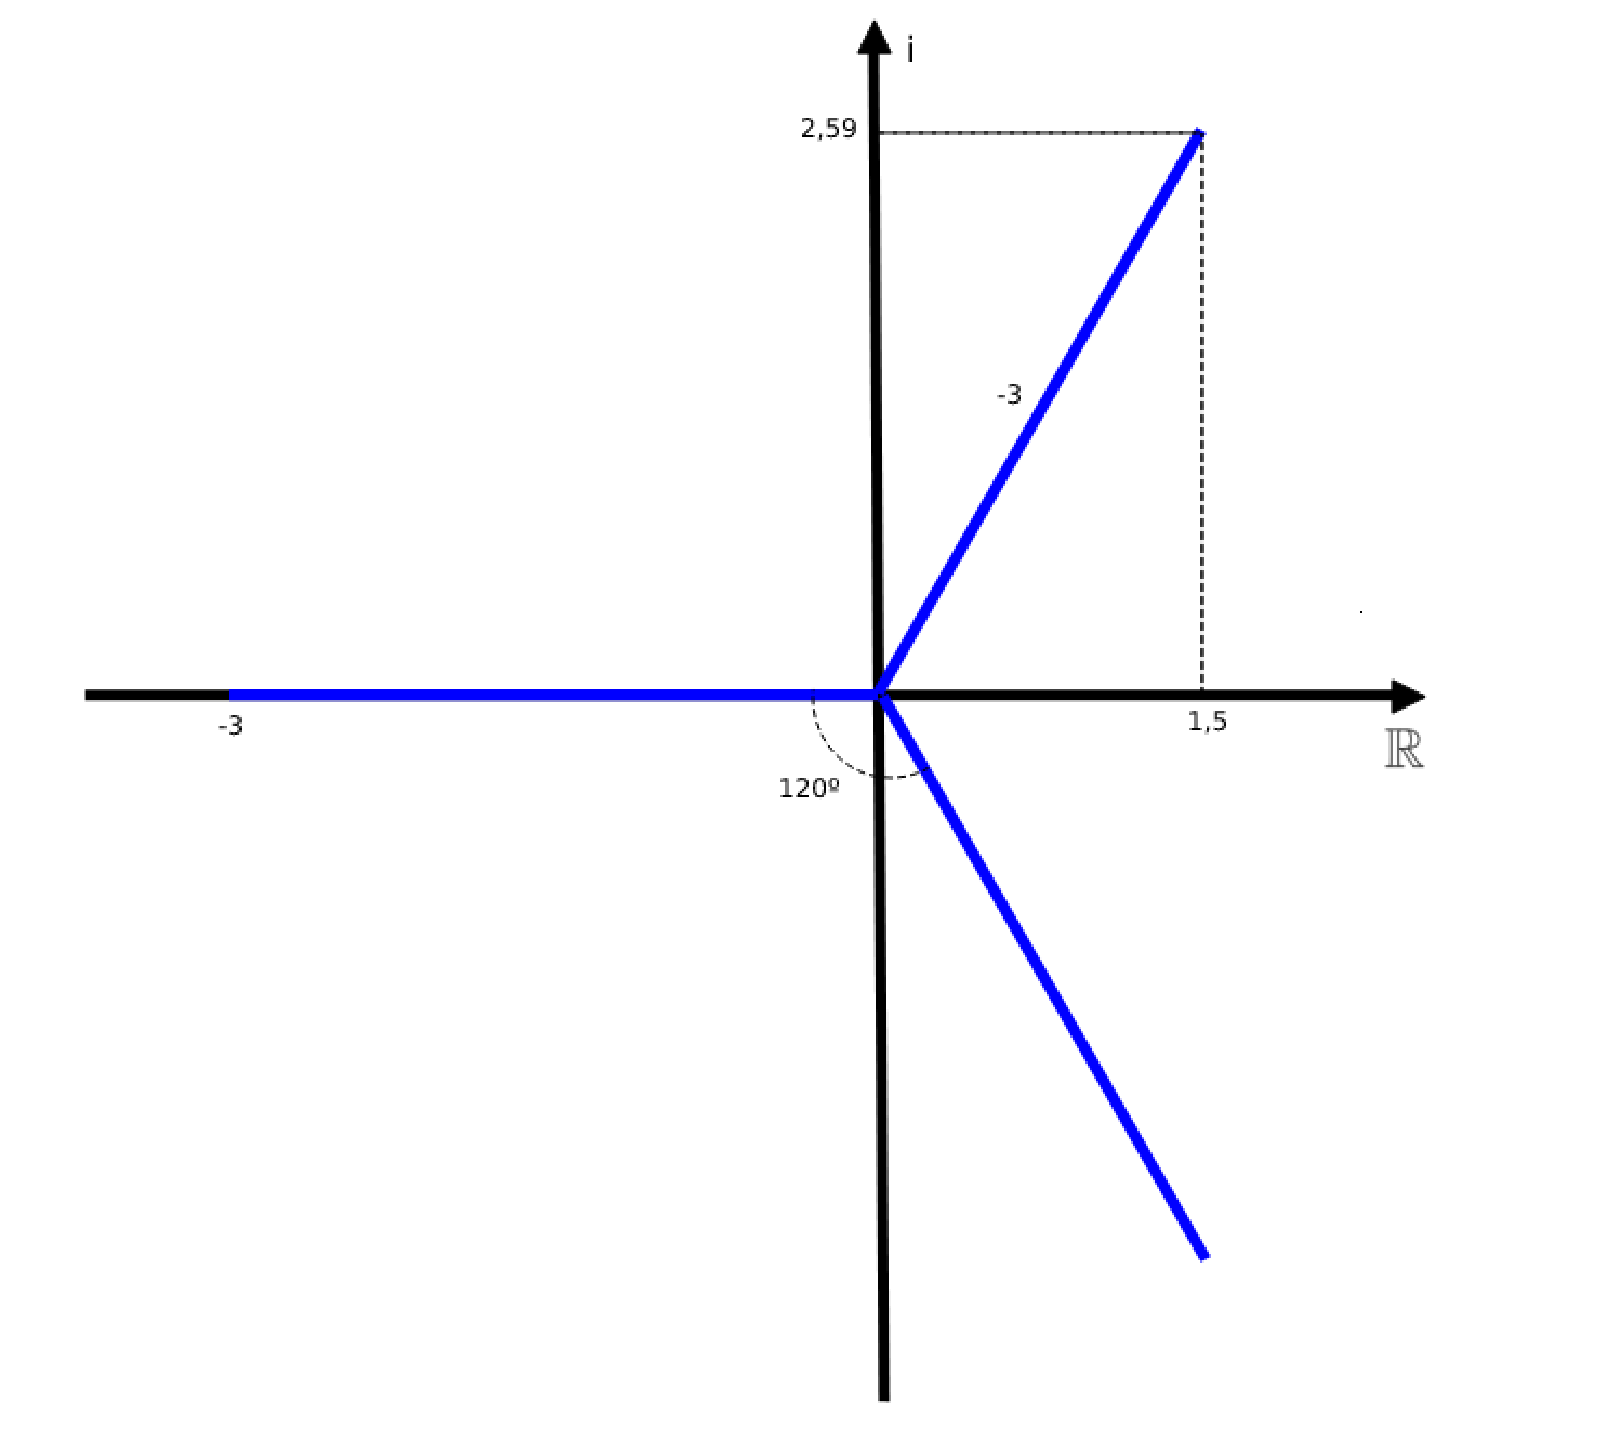
\includegraphics[width=\columnwidth]{image-roots-example.jpg}
    \caption{Ejemplificación de las soluciones complejas a una raíz.}
    \label{fig:roots_example}
\end{figure}

Para una mejor comprensión sobre el manejo de números complejos en Python, se sugiere consultar el estudio mencionado en ~\cite{b3}.

2. \textbf{Variable \( x_i \) igual a cero:} Aquí, el problema surge con los exponentes negativos, pues esta operación está indeterminada. Por tanto, para resolver este problema, utilizamos el valor absoluto del exponente, ya que al saber que la función a interpolar está definida en \( x_i = 0 \), podemos afirmar que \( e_j > 0 \).


\subsubsection{Fitness}
En esta sección, se realizará la evaluación de los cromosomas. Una idea fundamental en los algoritmos genéticos es la capacidad de valorar con la mayor precisión posible cada cromosoma, con el objetivo de determinar si un cromosoma es mejor o peor que otro. En el contexto de un problema de regresión, esta evaluación se basa en la comparación entre los valores predichos por el cromosoma y los valores reales.

Para evaluar la precisión de las predicciones, utilizamos el error cuadrático medio (RMSE, por sus siglas en inglés), una métrica ampliamente aceptada en problemas de regresión. El RMSE se calcula mediante la siguiente fórmula:

\[
\text{RMSE} = \sqrt{\frac{\sum_{i=1}^{N} (y_i - \hat{y}_i)^2}{N}}
\]


Una vez calculado el RMSE para un cromosoma específico, existen dos enfoques posibles para su utilización en la función de fitness: devolver el inverso del RMSE para maximizar el valor de la función de fitness, o devolver el RMSE directamente y minimizar su valor. En nuestro caso, hemos optado por la segunda opción, es decir, minimizar el RMSE.

A continuación, describiremos el proceso de predicción utilizando los datos del cromosoma en cuestión, que es crucial para la evaluación de su fitness.

\subsubsection{Predicción}
En esta sección, explicaremos cómo obtener una predicción \(\hat{y}_i\) para un cromosoma específico utilizando datos de prueba concretos. Este proceso se repetirá para cada uno de los datos de prueba que deseamos evaluar. Dado que estamos abordando un problema de regresión no lineal, debemos elevar cada una de las variables de los datos de prueba \(x_j\) a un exponente \(e_j\) y multiplicarlas por un coeficiente \(c_j\), donde \(j\) representa los índices de todas las variables en la ecuación de regresión. 

Posteriormente, sumamos estos términos junto con un último coeficiente, que actúa como término independiente, para obtener la predicción final. Utilizando los valores de un cromosoma determinado, la predicción \(\hat{y}_i\) se calcula de la siguiente manera:

\[
\hat{y}_i = \sum_{j=0}^{n} c_j x_j^{e_j} + c_{n+1}
\]


\subsubsection{Cruce de Cromosomas}
El proceso de cruce de cromosomas tiene como objetivo combinar dos cromosomas parentales, eligiendo uno o varios puntos de cruce de manera aleatoria. Una vez determinado el o los puntos de cruce, se crean dos cromosomas hijos seleccionando distintas parte de cada cromosoma padre. 

Consideramos la posibilidad de emplear uno o dos puntos de cruce en este proceso. Para tomar esta decisión, consultamos investigaciones previas sobre algoritmos genéticos (véase ~\cite{b1} y ~\cite{b2}). Sin embargo, finalmente llegamos a la conclusión de utilizar únicamente un punto de cruce. Esta elección se basa en nuestra consideración de que este enfoque se ajusta mejor a la documentación proporcionada y es una visión más sencilla y suficientemente eficaz para el problema a resolver.

Para decidir cuándo realizar el cruce, se utiliza una tasa de cruce, la cual es un valor entre 0 y 1. Se elige un número aleatorio, también entre 0 y 1, y la probabilidad de que este número sea menor que la tasa de cruce es precisamente la tasa de cruce. Por lo tanto, si el número aleatorio es mayor que la tasa de cruce, los cromosomas se devuelven sin cambios. 

En caso de que se deba realizar el cruce, se genera aleatoriamente un punto de corte en los cromosomas parentales. En este punto, ambos cromosomas se dividen y se combinan emparejando una mitad de uno con la mitad complementaria del otro, y viceversa. Podemos ver este proceso ejemplificado en \figurename~\ref{fig:chromosome-crossover}


\begin{figure}[H]
    \centering
    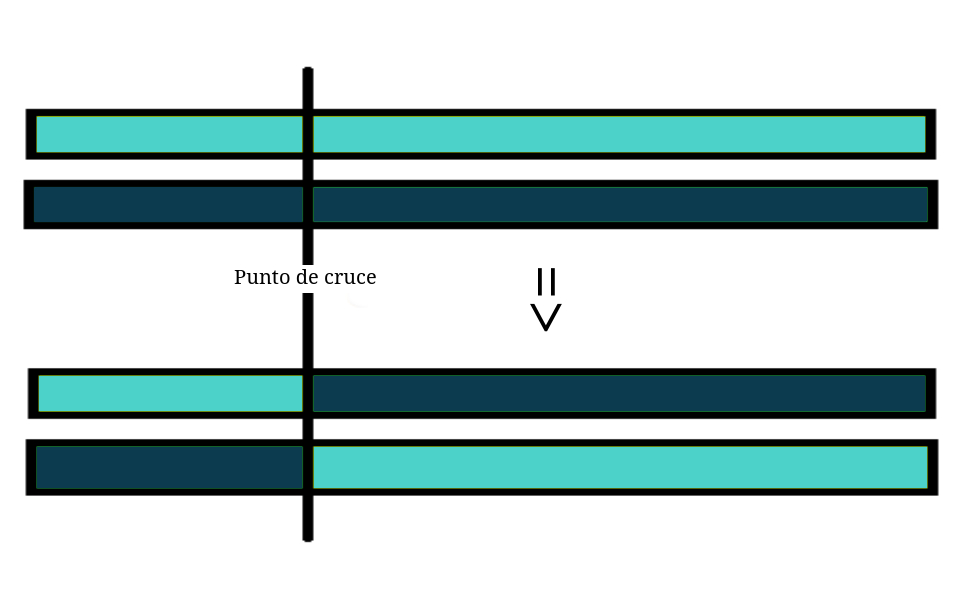
\includegraphics[width=\columnwidth]{image-chromosome-crossover.jpg}
    \caption{Proceso de cruce ilustrado.}
    \label{fig:chromosome-crossover}
\end{figure}


En nuestro caso, dado que manejamos dos listas, una de coeficientes y otra de exponentes, se generan dos puntos de corte y se realiza el cruce de la manera descrita anteriormente en ambas listas. Creando dos nuevos objetos Cromosoma, y devolviendo estos dos.



\subsubsection{Mutación de Cromosomas}
De primeras, contemplamos que la mutación de cromosomas se llevara a cabo de manera aleatoria, siguiendo un proceso similar al de cruce de cromosomas, pero, en este caso, generando un número aleatorio por cada parámetro del cromosoma a mutar.


Generando un número con el que determinar si un parámetro ha de ser mutado o no; cuando es seleccionado para mutación, se modifica sumándole o restando un valor aleatorio dentro de un rango predeterminado. Este rango incluye números negativos, lo que permite tanto el incremento como la disminución del parámetro con igual probabilidad. Y repitiendo este proceso para cada parámetro del cromosoma hasta completar el proceso de mutación.

Sin embargo, tras realizar diversas pruebas, observamos que se obtenían mejores resultados al generar un único número aleatorio y, en función de este, modificar de manera ligera todos los parámetros del cromosoma, en lugar de generar aleatoriedad para cada valor del cromosoma de forma individual. A pesar de que pueda parecer contraintuitivo, esta modificación no solo mejora el rendimiento, debido a la reducción en la generación de números y en las comprobaciones necesarias (lo cual es prácticamente insignificante), sino que también conduce a mejores resultados y a RMSE más reducidos.


\subsection{Algoritmo genético}
En esta sección, describimos el proceso completo del algoritmo genético, utilizando los componentes definidos anteriormente. El algoritmo comienza con la generación de una población inicial de un tamaño determinado. Cada cromosoma de la población es evaluado utilizando la función de fitness descrita previamente.

Una vez que todos los cromosomas han sido evaluados, se ordenan de menor a mayor según su valor de fitness, y se seleccionan los mejores para formar la población de la siguiente generación. Con los cromosomas restantes, se procede de la siguiente manera:

\subsubsection{Selección mediante torneo}
Para seleccionar los padres de la siguiente generación, se utiliza un método de selección mediante torneo. Este proceso consiste en seleccionar aleatoriamente \(k\) cromosomas y escoger los dos con mejor fitness, es decir, los dos con el menor RMSE respecto a los datos reales.

Una vez seleccionados los dos padres, se generan dos hijos para la siguiente generación utilizando el proceso de cruce explicado anteriormente. Posteriormente, estos hijos pasan por un proceso de mutación aleatoria. 

Este ciclo se repite tantas veces como el número de iteraciones especificado. Al finalizar la última iteración, se devuelve el cromosoma con el menor RMSE como la solución final al problema.


\subsection{Medidas para mejorar la eficiencia}
Además de buscar el menor RMSE posible, también teníamos la intención de optimizar los tiempos de ejecución de nuestro algoritmo, de manera que pudiera llegar a soluciones esperadas en el menor tiempo posible. Para alcanzar este objetivo, hemos implementado varias medidas destinadas a mejorar la eficiencia del algoritmo. Estas medidas son:

\subsubsection{Conjunto de datos para evaluar un cromosoma}

En principio, cuanto mayor sea el número de datos en nuestro conjunto de prueba, mejor será la valoración del cromosoma, ya que una mayor variedad de datos generalmente conduce a una regresión más precisa. Sin embargo, aumentar el número de casos de prueba también incrementa el tiempo necesario para evaluar cada cromosoma.

Para aprovechar las ventajas de disponer de un gran número de datos de prueba y, al mismo tiempo, reducir el costo computacional, propusimos la siguiente solución: introducir un nuevo parámetro, con un valor entre 0 y 1, que indique el porcentaje de datos a utilizar en cada valoración. Estos datos se seleccionarán de forma aleatoria para cada evaluación de un cromosoma. Sin embargo, esta idea presentaba un problema: en conjuntos de datos con un gran volumen de información, esta solución era beneficiosa, pero en aquellos con menor cantidad de datos, se perdía demasiada diversidad. Por lo tanto, consideramos que la mejor solución, sin necesidad de ajustar este valor en función del tamaño del conjunto de prueba, fue establecer un límite máximo de datos de prueba para cada proceso de evaluación. En conjuntos de entrenamiento con un número de datos menor que el límite, se utilizarían todos; mientras que en ficheros extensos se seleccionaría un subconjunto del tamaño de este límite, variando en cada proceso de evaluación de un cromosoma. En nuestro caso, hemos determinado que este límite de datos sea de 500 muestras.

De esta manera, un cromosoma que progresa a través de distintas generaciones debido a su buen desempeño en los datos asignados, será evaluado con diferentes subconjuntos de datos en cada iteración. Esto no solo asegura una evaluación más robusta, sino que también reduce significativamente el costo computacional de valorar un cromosoma.


\subsubsection{Almacenamiento de la valoración de un cromosoma}
Durante la ejecución del algoritmo genético, debemos ordenar todos los cromosomas de la población actual en función de su valoración. Estas valoraciones también se utilizan posteriormente en la selección por torneo.

Inicialmente, la población se representaba como una lista de cromosomas, y el cálculo de la valoración se realizaba cada vez que era necesario obtener la valoración de un cromosoma. Este enfoque era extremadamente ineficiente.

Para mejorar la eficiencia, propusimos cambiar esta lista de cromosomas por una lista en la que se almacenen pares \([\text{cromosoma}, \text{cromosoma.fitness()}]\). Consideramos varias opciones para implementar esta estructura, y finalmente optamos por utilizar una lista de listas. Aunque esta elección podría ser ligeramente menos eficiente que usar un diccionario o una lista de tuplas, vimos que la manipulación de listas era lo más comodo para nosotros. Las listas son variables mutables, lo que nos permite crear la población de la siguiente generación y realizar operaciones de mutación y cruce con facilidad. Al comienzo de cada nueva generación, podemos establecer las valoraciones utilizando nuevos datos de prueba, tal como se explicó anteriormente.


\section{Metodología}

Esta sección presenta los pseudocódigos de cada una de las funciones que se usan en el diseño del algoritmo genético, los cuales han sido explicados en el apartado \ref{sec: preliminares}.


\begin{figure}[H]
  \centering
  \begin{pseudo}*
    \hd{\fn{fitness}}(self, train\_data, data\_percentage) \\*
    \multicolumn{2}{l}{\textbf{Entrada}: El cromosoma actual, una lista de tuplas de} \\*
    \multicolumn{2}{l}{floats que representan los datos de entrenamiento y un} \\*
    \multicolumn{2}{l}{ float que representa el porcentaje de datos con los que} \\*
    \multicolumn{2}{l}{ será entrenado el cromosoma} \\*
    \multicolumn{2}{l}{\textbf{Salida}: Un float que representa el error cuadrático medio} \\*
    \multicolumn{2}{l}{ (RMSE)} \\
    \fn{predicted \(\leftarrow\) lista vacía} \\
    \fn{expected \(\leftarrow\) lista vacía} \\
    \fn{subset \(\leftarrow\)} seleccionar aleatoriamente \\+
    \fn{(train\_data * data\_percentage) elementos de} \\+
    \fn{train\_data} \\--
    \textbf{para cada} \fn{datum} \textbf{en} \fn{subset} \textbf{hacer} \\+
    agregar \fn{llamada a la funcion predict con datum} \\+ \fn{como parametro} a \fn{predicted} \\
    agregar \fn{último elemento de datum} a \fn{expected} \\-
    \fn {rmse} \(\leftarrow\) \fn{root\_mean\_squared\_error}(expected, predicted) \\
    \textbf{devolver} \fn{rmse}
  \end{pseudo}
  \caption{Función de evaluación del cromosoma (\texttt{fitness}) en pseudocódigo}
  \label{pcd:fitness}
\end{figure}


\begin{figure}[H]
  \centering
  \begin{pseudo}*
    \hd{\fn{predict}}(\textit{self, datum}) \\*
    \multicolumn{2}{l}{\textbf{Entrada}: El cromosoma actual, una tupla de floats que} \\*
    \multicolumn{2}{l}{representa una línea de los datos de entrenamiento} \\*
    \multicolumn{2}{l}{\textbf{Salida}: Un float que representa el valor predicho} \\
    \fn{prediction \(\leftarrow\) 0} \\
    \textbf{para cada} \fn{j} \textbf{en rango} \fn{len(datum) - 1} \textbf{hacer} \\+
    
    \textbf{si} \fn{\textit{el dato recibido j}} es igual que \fn0 \textbf{entonces} \\+
    \textit{\fn{el exponente j}} \(\leftarrow\) \fn{hacer el valor absoluto} \\-
    \fn{power\_term \(\leftarrow\) \textit{sign de datum j * modulo de }} \\+
    \fn{(datum j ** exponente j)} \\-
    \fn{prediction} \(\mathrel{+}= \textit{\fn{el coeficiente j}} \times \fn{\textit{power\_term }} \\-
    \fn{prediction} \(\mathrel{+}= \textit{ \fn{término independiente}}\) \\
    \textbf{devolver} \fn{prediction}
  \end{pseudo}
  \caption{Función de predicción (\texttt{predict}) en pseudocódigo}
  \label{pcd:predict}
\end{figure}



\begin{figure}[H]
  \centering
  \begin{pseudo}*
    \hd{\fn{crossover}}(\textit{self}, \textit{ parent1, parent2}, \textit{cross\_rate}) \\*
    \multicolumn{2}{l}{\textbf{Entrada}: Padre1, padre2 y la tasa de cruce} \\*
    \multicolumn{2}{l}{\textbf{Salida}: Una lista de los dos cromosomas resultantes} \\
    \textbf{si \fn{el número random generado} es mayor que} \textit{\fn{cross\_rate}} \\+
    \textbf{entonces} \\+
    \textbf{devolver \fn{una lista con parent1 y parent2}} \\+
    \fn{cromosoma con el que iba a ser cruzado} \\---
    \fn{point} \(\leftarrow\) \fn{número random entre el uno y la longitud de } \\+
    \fn{la lista de exponentes de parent1 menos uno} \\---
    \fn{child1\_coefficients} \(\leftarrow\)
    \textit{\fn{los coeficientes}} \\+ 
    \textit{\fn{de parent1 hasta "punto" + los coeficientes de }} \\+
     \textit{\fn{parent2 desde "punto"}} \\--
    \fn{child1\_exponents} \(\leftarrow\)
    \textit{\fn{los exponentes de parent1}} \\+ 
    \textit{\fn{ hasta "punto" + los exponentes de }} \\+
     \textit{\fn{parent2 desde "punto"}} \\--
     \fn{child2\_coefficients} \(\leftarrow\) \textit{\fn{los coeficientes de parent2}} \\+ 
    \textit{\fn{ hasta "punto" + los coeficientes de }} \\+
     \textit{\fn{parent1 desde "punto"}} \\--
    \fn{child2\_exponents} \(\leftarrow\)
    \textit{\fn{los exponentes de parent2}} \\+ 
    \textit{\fn{ hasta "punto" + los exponentes de }} \\+
     \textit{\fn{parent1 desde "punto"}} \\--
    \textbf{devolver} \fn{lista con el cromosoma child1\_coefficients} \\+
    \fn{y child1\_exponents, y el cromosoma } \\+
    \fn{child2\_coefficients y child2\_exponents}
  \end{pseudo}
  \caption{Función de cruza (\texttt{crossover}) en pseudocódigo}
  \label{pcd:crossover}
\end{figure}


\begin{figure}[H]
  \centering
  \begin{pseudo}*
    \hd{\fn{mutate}}(\textit{self}, \textit{mutation\_rate}, \textit{mutation\_range}) \\*
    \multicolumn{2}{l}{\textbf{Entrada}: El cromosoma actual, tasa de mutación y rango de} \\*
     \multicolumn{2}{l}{mutación} \\*
    \multicolumn{2}{l}{\textbf{Salida}: Ninguna} \\
    \textit{\fn{random\_number}} \(\leftarrow\) \fn{Número aleatorio entre 0 y 1} \\--
    \textbf{si} \textit{\fn{random\_number} es menor que}  \textit{\fn{mutation\_rate}} \textbf{entonces} \\+
        \textbf{para cada} \textit{\fn{i}} \textbf{en rango} \fn{longitud de la lista de exponentes} \\+
        \fn{ del cromosoma actual }\textbf{hacer} \\+
            \textit{\fn{coeficiente i del cromosoma actual}}  \fn{ += un valor}\\+
            \fn{aleatorio entre -mutation\_range y} \\+ \fn{mutation\_range}\ \\--
            \textit{\fn{exponente i del cromosoma actual}} \fn{ += un valor}\\+
            \fn{aleatorio entre -mutation\_range y} \\+ \fn{mutation\_range}\ \\----
        \textit{\fn{último coeficiente del cromosoma actual}} \fn{+= un valor}\\+
            \fn{aleatorio entre -mutation\_range y mutation\_range}\\--
  \end{pseudo}
  \caption{Función de mutación (\texttt{mutate}) en pseudocódigo}
  \label{pcd:mutate}
\end{figure}


\begin{figure}[H]
  \centering
  \begin{pseudo}*
    \hd{\fn{tournament\_selection}}(\textit{self}, \textit{k}) \\*
    \multicolumn{2}{l}{\textbf{Entrada}: Instancia de la clase AG y número de cromosomas} \\*
    \multicolumn{2}{l}{seleccionados para el torneo (\textit{k})} \\*
    \multicolumn{2}{l}{\textbf{Salida}: Cromosoma con la mejor aptitud} \\
    \textit{\fn{tournament}} \(\leftarrow\) \fn{k elementos aleatorios de población actual}\\---
    \textbf{devolver} \textit{\fn{ elemento con menor fitness}} \\
  \end{pseudo}
  \caption{Selección de torneo en pseudocódigo}
  \label{pcd:tournament_selection}
\end{figure}




\begin{figure}[H]
  \centering
  \begin{pseudo}*
    \hd{\fn{test}}(\textit{self}, \textit{chromosome}) \\*
    \multicolumn{2}{l}{\textbf{Entrada}: Instancia de la clase AG y cromosoma a probar} \\*
    \multicolumn{2}{l}{\textbf{Salida}: Lista de valores predichos} \\
    \textbf{devolver} \textit{\fn{[predicción \textbf{de} dato \textbf{por} dato \textbf{en} conjunto de test]}} \\
  \end{pseudo}
  \caption{Función de prueba (\texttt{test}) en pseudocódigo}
  \label{pcd:test}
\end{figure}




\begin{figure}[H]
  \centering
  \begin{pseudo}*
    \hd{\fn{run}}(\textit{self}) \\*
    \multicolumn{2}{l}{\textbf{Entrada}: Instancia de la clase AG} \\*
    \multicolumn{2}{l}{\textbf{Salida}: El cromosoma con la mejor aptitud encontrada y ese} \\*
    \multicolumn{2}{l}{cromosoma sometido a la funcion test} \\
    \textit{\fn{elitism\_count}} \(\leftarrow\) 
    \fn{ratio de elitismo por el tamaño de} \\+
    \textit{\fn{población}}\\--
    \textbf{para} \textit{\fn{generation}} \textbf{en rango} \textit{\fn{máximas iteraciones}} \textbf{hacer} \\+
    \textbf{para} \textit{\fn{pair}} \textbf{en} \textit{\fn{la población actual}} \textbf{hacer} \\+
        \textit{\fn{self.population}} \(\leftarrow\) 
        \fn{lista de listas del primer} \\+
        \fn{elemento de pair y de su función fitness} \\--
        \textit{\fn{self.population}} \(\leftarrow\) 
        \fn{se ordena por el segundo}\\+
        \fn{elemento de cada tupla de la lista de}\\+
        \fn{población} \\--
        \textbf{para} \textit{\fn{pair}} \textbf{en} \textit{\fn{la población actual hasta el}} \\+
        \fn{elitism\_count elemento} \textbf{hacer} \\+
        \textit{\fn{next\_generation}} \(\leftarrow\) \fn{añadir el primer} \\+
        \fn{elemento de pair} \\---
        \textbf{mientras} \fn{longitud de}
        \textit{\fn{next\_generation} menor que} \\+
        \textit{\fn{tamaño de población}} \textbf{hacer} \\+
            \fn{\textit{parent1}, \textit{parent2}} \(\leftarrow\) \fn{cromosoma ganador} \\+
            \fn{\textit{del torneo} \textit{cromosoma ganador del}} \\+
            \textit{torneo} \\--
            \textit{\fn{offspring}} \(\leftarrow\) \textit{\fn{crossover entre parent 1 y 2}}\\
            \textbf{para cada} \textit{\fn{child}} \textbf{en} \textit{\fn{offspring}} \textbf{hacer} \\+
                \textbf{si} \fn{longitud de next\_generation} menor\\+
                que \fn{tamaño población} \\+
                    \fn{\textit{child} \(\leftarrow\) \textit{mutate cromosoma}} \\
                    \fn{\textit{next\_generation}} \(\leftarrow\) \textit{añadir}\\+ \fn{child} \\------
        \fn{\textit{best\_fitness} \(\leftarrow\) \textit{segundo elemento de la primera tupla}}\\+
        \fn{de la lista de población} \\-
        \fn{\textit{self.population} \(\leftarrow\) \textit{next\_generation}} \\-
    \textit{\fn{winner\_chromosome}} \(\leftarrow\) 
    \fn{cromosoma con mejor fitness}\\
    \textbf{devolver} 
    \fn{\textit{winner\_chromosome}, \textit{test de winner\_chromosome}} \\
  \end{pseudo}
  \caption{Función de ejecución (\texttt{run}) en pseudocódigo}
  \label{pcd:run}
\end{figure}









\section{Resultados}

En esta sección se presentan los resultados del entrenamiento del modelo de regresión no lineal utilizando algoritmos genéticos. Para ello, se emplearon tres conjuntos de datos distintos: \texttt{toy1}, \texttt{housing} y \texttt{synt1}. El modelo fue entrenado y evaluado de manera independiente para cada conjunto de datos, utilizando un archivo de prueba específico para cada caso.

El tiempo de entrenamiento varía significativamente según el conjunto de datos aplicado. Los principales factores que influyen en el tiempo de entrenamiento son los siguientes:

\begin{itemize}
    \item \textbf{Tamaño del conjunto de entrenamiento}: Este factor se refiere a la cantidad de datos disponibles para entrenar el modelo. En nuestro caso, su impacto es menor debido a la decisión de diseño de utilizar un conjunto de entrenamiento dinámico a lo largo de las diferentes generaciones del algoritmo, tal como se describe en la sección de mejoras de optimización.
    
    \item \textbf{Número de variables del conjunto de datos}: Este es un factor crucial, ya que un mayor número de variables ralentiza el proceso de predicción, el cual debe repetirse numerosas veces durante el entrenamiento. En particular, este factor es determinante para el tiempo de entrenamiento del conjunto de datos \texttt{synt1}.
\end{itemize}

Una vez entrenado el modelo, y antes de devolver el cromosoma óptimo, se evalúa su desempeño utilizando un conjunto de datos de prueba. Este conjunto permite determinar la eficacia del modelo. Tras esta evaluación, se selecciona el cromosoma ganador y se generan las predicciones \(\hat{y}_i\) para todos los datos del conjunto de prueba. A continuación, se calcula el Error Cuadrático Medio (RMSE) entre los resultados esperados y los obtenidos, así como el coeficiente de determinación (\(R^2\)).

Durante todo este proceso, tanto en la fase de entrenamiento como en la de prueba, se inicia un temporizador para medir el tiempo total empleado en el modelado de la solución, siendo este uno de los datos clave reportados.

Es importante destacar que, aunque varios procesos dentro del algoritmo, como la mutación, el cruce y la asignación de datos a cada cromosoma, son inherentemente aleatorios, estos procesos se controlan mediante una semilla específica. Esta semilla, proporcionada por la librería de Python utilizada, asegura que el experimento es reproducible. Por lo tanto, si el programa se ejecuta múltiples veces sin cambiar ningún parámetro, los resultados serán consistentes. Para obtener diferentes resultados con los mismos parámetros, es necesario modificar la semilla.

Los parámetros que influyen en los posibles resultados del modelo son los siguientes: tamaño de la población de cromosomas, número de iteraciones (aunque otra forma de limitar el proceso podría ser alcanzar un RMSE determinado o un tiempo máximo especificado), tasa de mutación, rango de mutación (el intervalo en el que se encuentra el valor que se va a sumar o restar a las posiciones del cromosoma), rango de valores iniciales, tasa de cruce y tasa de elitismo. En nuestro estudio, los valores seleccionados para estos parámetros son:

\begin{table}[H]
\centering
\caption{Parámetros del modelo y sus valores.}
\label{tab:parametros}
\begin{tabular}{ll}
\toprule
\textbf{Parámetro} & \textbf{Valor} \\
\midrule
Tamaño de la población         & 50 \\
Número de iteraciones          & 300 \\
Tasa de mutación               & 0.2 \\
Rango de mutación              & 0.6 \\
Rango de valores iniciales     & 1.0 \\
Tasa de cruce                  & 0.7 \\
Tasa de elitismo               & 0.2 \\
\bottomrule
\end{tabular}
\end{table}


Es importante destacar que todos estos parámetros pueden afectar de manera tanto positiva como negativa a los resultados obtenidos. Lo que puede ser beneficioso para un conjunto de datos podría resultar perjudicial para otro. Por este motivo, hemos seleccionado valores que buscamos que sean adecuados para todos los conjuntos de datos empleados. No obstante, se recomienda ajustar estos parámetros según sea necesario para optimizar los resultados en un conjunto de datos específico. Estos parámetros pueden ser establecidos al crear la instancia del \texttt{AG} mediante los \texttt{**kwargs} del constructor.

El tiempo del algoritmo depende de, entre otras cosas, el equipo en el que se prueba (tanto hardware como software); en nuestro caso lo hemos probado en dos sistemas, estos son:
\textbf{Sistema 1}
\begin{itemize}
    \item \textbf{CPU}: \textit{AMD Ryzen 7 7000 Series}
    \item \textbf{Sistema operativo}: \textit{Linux Fedora}
    \item \textbf{Terminal}: \textit{Warp}
\end{itemize}


\textbf{Sistema 2}
\begin{itemize}
    \item \textbf{CPU}: \textit{Intel i7 10510U}
    \item \textbf{Sistema operativo}: \textit{Windows 11}
    \item \textbf{Terminal}: \textit{Powershell}
\end{itemize}
Recomendamos lanzarlo desde una terminal lo más optimizada posible, en lugar de la incorporada en un IDE.

Con los parámetros establecidos, los resultados obtenidos para cada fichero se presentan en la Tabla~\ref{tab:resultados1} para el primer sistema y en la Tabla ~\ref{tab:resultados2} para el segundo. 

Además, hemos implementado un sistema de registros que, de manera dinámica, actualiza los mejores valores obtenidos a medida que se prueban distintos parámetros o se cambian las semillas. Este registro puede consultarse en \textit{./data/log.txt}, partiendo del directorio raíz del proyecto una vez descomprimido.

Para ejecutar el proyecto, ofrecemos dos opciones: 
\begin{enumerate}
    \item Lanzar el proyecto sin parámetros, utilizando el comando: \textit{python ./src/prueba\_AG.py}, que empleará el fichero predeterminado, en este caso \textit{toy1}. Este fichero predeterminado puede ser modificado manualmente en el archivo \textit{prueba\_AG.py}, como se indicó en la plantilla proporcionada.

    \item Modificar el fichero de manera más conveniente añadiendo el nombre del fichero como argumento en la línea de comandos: \textit{python ./src/prueba\_AG.py nombre\_fichero}. Los nombres de fichero válidos son: \textit{toy1}, \textit{housing} y \textit{synt1}.
\end{enumerate}


Para cualquier duda sobre la instalación de dependencias o la configuración correcta del proyecto, consulte el archivo \textit{README.md} incluido en el directorio raíz del proyecto.


\begin{table} [H]
  \caption{Resultados obtenidos sistema 1}
  \label{tab:resultados1}
  \centering
  \begin{tabular}{cccc}
    \toprule
     Fichero & Toy1 & Housing & Synt1 \\
    \midrule
    RMSE & 0.3417 & 0.7564 & 190.8364 \\
    R2 & 0.9436 & 0.5739 & -0.0474 \\
    \midrule
    Tiempo & 6.62 & 20.61 & 160.97 \\
    Seed & 123 & 124 & 123 \\
    \bottomrule
  \end{tabular}
\end{table}

\begin{table} [H]
  \caption{Resultados obtenidos sistema 2}
  \label{tab:resultados1}
  \centering
  \begin{tabular}{cccc}
    \toprule
     Fichero & Toy1 & Housing & Synt1 \\
    \midrule
    RMSE & 0.3517 & 0.7564 & 190.8364 \\
    R2 & 0.9403 & 0.5739 & -0.0474 \\
    \midrule
    Tiempo & 16.29 & 49.65 & 487.17 \\
    Seed & 123 & 124 & 123 \\
    \bottomrule
  \end{tabular}
\end{table}


\section{Conclusiones}

En este proyecto, se ha desarrollado y evaluado un modelo de regresión no lineal utilizando algoritmos genéticos. La metodología incluyó la representación de coeficientes y exponentes en cromosomas, la aplicación de operadores genéticos como mutación y cruce, y la evaluación de la aptitud utilizando el error cuadrático medio (RMSE). Se realizaron experimentos con tres conjuntos de datos distintos: \texttt{toy1}, \texttt{housing} y \texttt{synt1}. Los resultados mostraron una mejora significativa en la precisión de las predicciones al optimizar el manejo de los números complejos con el uso de los modulos de estos, y en la velocidad de rendimiento al usar un límite de ejemplos en el entrenamiento y el almacenamiento de la valoracion de los cromosomas durante el algoritmo.

Los experimentos demostraron que el tiempo de entrenamiento varía según el tamaño del conjunto de datos y el número de variables. En particular, el conjunto de datos \texttt{synt1} presentó mayores desafíos debido a su complejidad, por lo que cualquier cambio podía suponer una diferencia notable en los resultados de este fichero. Para poder obtener los mejores resultados posibles, se llevo a cabo la implementación de un sistema de registro de records además del control de la semilla de aleatoriedad que aseguraron la reproducibilidad de los resultados más óptimos.

Para futuros trabajos, se sugiere una serie de mejoras y exploraciones adicionales. Entre estas mejoras, la paralelización de partes del código podría mejorar significativamente el rendimiento del algoritmo genético. La optimización de parámetros del algoritmo genético, como las tasas de mutación y cruce, y la incorporación de métodos avanzados de selección también podría conducir a mejoras adicionales en la precisión y eficiencia del modelo. Finalmente, sería beneficioso explorar la aplicación de este enfoque en otros dominios y con conjuntos de datos más grandes y complejos para validar su generalizabilidad y robustez.


\begin{thebibliography}{00}
\bibitem{b1}Mathew, Tom V. "Genetic algorithm." Report submitted at IIT Bombay 53 (2012), pp 7-8.

\bibitem{b2}Pose, Marcos Gestal. "Introducción a los algoritmos genéticos." Departamento de Tecnologías de la Información y las Comunicaciones Universidad de Coruña (2000).

\bibitem{b3}van Rossum, G., and Drake, F. L. (Eds.). (2006). An introduction to Python. Network Theory Limited, pp 15-18.

\bibitem{b4}https://scsynth.org/t/fractional-powers-of-negative-numbers/4224
\end{thebibliography}




\end{document}
